\newpage
\section{Principe}

Le programme à paralléliser est déjà fourni, il est donc nécessaire d'en comprendre un minimum le fonctionnement pour déterminer ce qui pourra être paralléliser ou non. Le but du programme est de reconstituer une scène du point de vue d'un oeil/d'une caméra, en utilisant un algorithme de lancer de rayons. D'après le principe de retour inverse, en faisant partir des rayons depuis l'oeil dans toute les directions, et en leur appliquant les lois de réflexion et de réfraction, on obtient la scène reconstituée telle qu'elle est vue par l'oeil. Ainsi, en lançant un rayon pour chaque \emph{pixel} de l'image désirée, le programme parvient à reconstituer la scène. Tous ces lancers sont indépendants les uns des autres car seules les lectures de la scène sont communes, pas les écritures des \emph{pixels}. Tous ces calculs peuvent donc être parallélisés.

La complexité du calcul pour un \emph{pixel} donné dépend des réflexions/réfractions que le rayon associé va subir, ce qui est lié aux objets qu'il va rencontrer. Comme les objets ont généralement des aspects contigus, on peut en déduire que si le rayon associé à un \emph{pixel} rencontre un objet, alors les rayons associés aux \emph{pixels} voisins vont sûrement rencontrer ce même objet. Ainsi, le temps de calcul pour un \emph{pixel} donné à de forte chance d'être proche de celui de ses voisins. C'est pour cela que le sujet introduit la notion de tuile qui sont des carrés de plusieurs \emph{pixels} ($8\times8$ ou $16\times16$) à traiter d'un coup.

\subsection{Parallélisation}

Les carrés de \emph{pixels}, que nous appellerons des tuiles sont la brique de base du projet : ce sont les calculs de rendus des tuiles que nous souhaitons paralléliser (au sein d'une image, plusieurs tuiles peuvent donc être calculées en même temps, mais au sein d'une tuile pas plusieurs \emph{pixels}. Différentes répartitions de ces tuiles sont envisagées, elles sont explicitées ci-dessous. 

Les notations suivantes seront utilisées par la suite : $P$ le nombre de processus, et $C$ le nombre de tuiles, numérotées de 0 à $C-1$ de gauche à droite et de haut en bas. De plus $q$ est la partie entière supérieure de la division de $C$ par $P$ ($q = \frac{C+P-1}{P}$).

\subsubsection*{Répartition statique}

Une première idée consiste à attribuer au processus $i$ le traitement des tuiles numérotées entre $i\times q$ et $(i+1)\times q - 1$ (sauf le dernier processus, qui va jusqu'à $C-1$). L'inconvénient est que les processus ont à traiter des tuiles contiguës, or comme les temps d'exécution ont une forte probabilité d'être similaire pour des tuiles voisines, il y a alors un fort risque de mauvais équilibrage de charge si un processus récupère des tuiles demandant beaucoup plus de temps de calcul que les autres (correspondant à une partie de l'image comportant beaucoup de mirois par exemple).

Afin de prévenir ce problème, le théorème des restes chinois est utilisé pour répartir les tuiles (d'une façon plutôt aléatoire, mais garantissant un nombre de tuiles à traiter du même ordre pour chaque processus) sur tous les processus. On attribue alors au processus $i$ les tuiles $tuiles(i) = {(j\times N)\% C, j\in \llbracket i\times q, min((i+1)\times q - 1, C-1)\rrbracket}$. Le théorème des restes chinois nous garantit que lorsque j parcourt $\llbracket 0, C-1\rrbracket$, $tuiles(i)$ parcourt également $\llbracket 0, C-1\rrbracket$.

\subsubsection*{Répartition dynamique}

La répartition statique ne garantit toutefois toujours pas que les charges de calcul sont bien distribuées, certaines tuiles demandant beaucoup plus de temps que d'autres. Il apparaît donc convenable de se pencher sur une distribution dynamique des tuiles, afin de pallier les lacunes de la distribution statique en réattribuant des tuiles au cours de l'exécution.

Le concept abordé est celui du vol de travail. Une première distribution de tuiles (statique) a lieu en début de programme, à l'issue de laquelle chaque processus possède un certain nombre de tâches à exécuter, lesquelles sont stockées dans une pile locale. Lorsqu'un processus arrive au terme de sa pile de tâches, il va d'aller chercher du travail chez ses voisins, à condition que ses derniers ne soient pas non plus en rupture de stock.

\subsection{Architecture de l'ensemble des processus}

Il a été décidé d'organiser les processus en un cercle de communication, notamment dans le but d'organiser le vol de tâches. Cela a pour avantage principal le fait que les messages passent par tous les processus et sont donc visibles de tous (ce qui est utile pour prévenir tous les processus, par exemple pour la terminaison du programme) en évitant d'avoir à effectuer des \emph{broadcasts} qui sont très coûteux. De plus, cela simplifie les communications car l'essentiel d'entre elles se font avec les voisins directs.

Dans notre cas, on oriente le cercle, ainsi chaque processus a un prédécesseur et un successeur. Les communications se font toujours du processus vers son successeur.

\subsubsection*{Les messages}

Initialement trois types de messages ont été défini pour la communication entre processus. Ces types de messages correspondent aux étiquettes de l'automate associé au protocole de communication entre les processus, représenté dans la figure \ref{img:old_automate}.

\begin{figure}
\raggedright
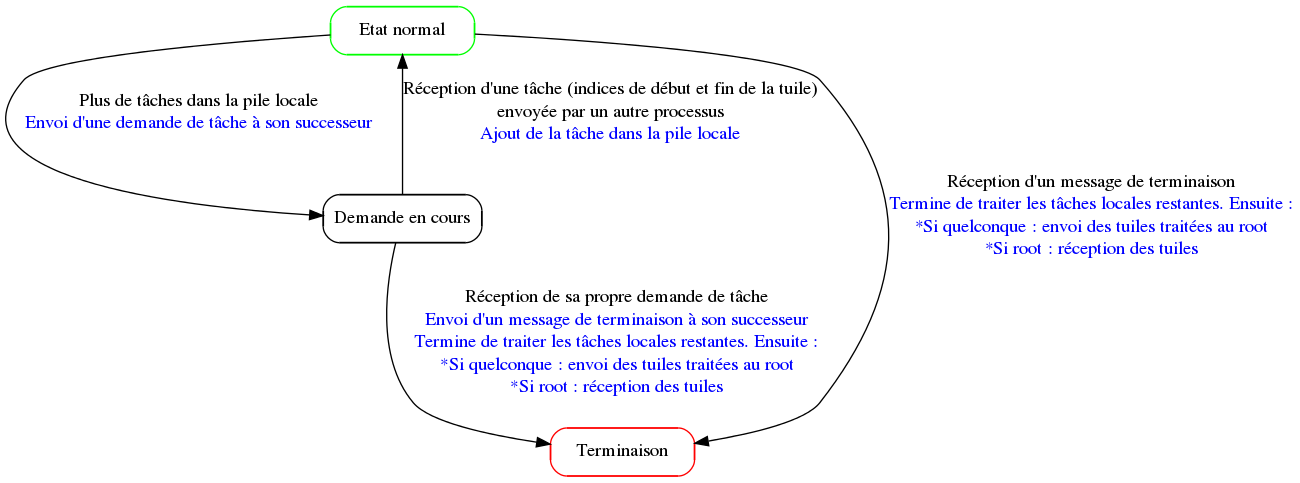
\includegraphics[scale=0.4]{old_automate.png}
\caption{Automate de communication, à 3 états et 3 étiquettes.}
\label{img:old_automate}
\end{figure}

\paragraph{ASK}
C'est le message qu'envoie un processus lorsqu'il n'a plus de tuiles à traiter. Il envoie ce message à son successeur. Lorsqu'un processus reçoit un message de ce type, il y a trois cas possibles :
\begin{itemize}
\item[$\bullet$]Dans le cas particulier où l'émetteur originel du message est le processus lui-même, alors le message a fait le tour du cercle sans que personne ne réponde, signifiant que les processus n'ont plus de travail à partager. Il convient donc de lancer la terminaison de l'exécution, ce qui est fait en envoyant un message de terminaison (\textbf{END}).
\item[$\bullet$]Sinon, si le processus a des tâches à fournir, il va directement contacter le processus demandeur pour lui envoyer une tuile à traiter (message \textbf{TILE}).
\item[$\bullet$]Enfin, si le processus n'a pas de travail à partager, alors il va se contenter de transmettre le message à son successeur.
\end{itemize}
%\vspace{0.3cm}

\paragraph{TILE}
Ce type de message est destiné à transférer une tuile d'un processus à un autre. Le message a pour source un processus qui a au moins une tâche à partager, et a pour destination un processus demandeur de travail. C'est le seul message qui est communiqué sans prendre en compte l'architecture en cercle. Il peut contenir une ou plusieurs tuiles, nous avons choisi d'envoyer $1$ tuile s'il n'en reste pas beaucoup au processus émetteur, ou $NB\_THREADS$ s'il lui en reste suffisamment, afin d'occuper tous les \emph{threads} du récepteurs.

\paragraph{END}
Ce message a pour fonction de prévenir l'ensemble des processus que le programme entre dans sa phase de terminaison. Si un processus qui le reçoit n'en est pas l'émetteur originel, alors il le fait suivre car il y a potentiellement des processus entre lui et l'émetteur, qui n'auraient donc pas reçu le message. Dans le cas contraire, alors le message a fait le tour du cercle et donc le renvoyer n'a aucune utilité : dès que les tâches en cours seront terminées, tous les \emph{threads} ainsi que la communication en anneau s'arrêteront.

\subsubsection*{Seconde version des messages}

L'automate précédent, avec les messages associés, peut amener à un \emph{deadlock}. Ce cas peut se produire lorsque le processus racine est prévenu de la terminaison après que d'autres processus ont terminés et ont commencé à lui envoyer leurs tuiles directement (sans passer par l'anneau de communication). Le \emph{thread} de communication reçoit alors un message qu'il ne sait pas traiter, et pour lequel il n'effectue donc pas la réception. Ce message reste en tête de la pile, au-dessus des messages de terminaisons, et bloque donc l'avancée des communications. 

Deux solutions ont alors été envisagées pour pallier ce problème. Toutes les deux nécessitent une terminaison en deux temps : une première phase pour que tout le monde jusqu'à la racine soit prévenu d'une demande de terminaison, une seconde pour que la racine autorise la terminaison. 
\begin{itemize}
\item[$\bullet$] La première solution consiste à ne pas terminer le \emph{thread} de communication tant que l'on a pas reçu un message de confirmation par la racine (cette réception bloquante est donc effectuée après la transmission du message de terminaison au successeur, et avant le \texttt{return} du \emph{thread} de communication. Le processus racine, quand il reçoit une demande de terminaison, effectue quant à lui un envoi du message de terminaison définitive vers chaque autre processus puis termine. Cette solution s'apparente toutefois à un \emph{broadcast} et n'est pas dans l'esprit de l'anneau de communication.
\item[$\bullet$] La seconde solution, celle actuellement dans le code (l'autre étant en commentaire), nécessite deux tours de l'anneau de communication pour terminer. D'abord un processus quelconque (y compris la racine) envoi une demande de terminaison qui est transmise jusqu'à la racine. Une fois que la racine l'a reçu, elle envoi un message de terminaison définitive : chaque processus la transmet au successeur puis termine. Certains messages sont donc perdus, et cette solution est inévitablement plus lente.
\end{itemize}

Le nouvel automate associé à cette nouvelle solution est représenté par la figure \ref{img:automate}. Il comprend la nouvelle étiquette \textbf{FINISH}\footnote{Cette étiquette existait déjà dans la version originale, mais n'était utilisé qu'une fois que tous les \emph{threads} étaient censés avoir terminés, ce qui n'était pas tout le temps le cas et conduisait au \emph{deadlock} découvert sur \textsf{Plafrim}.} qui est à traduire par \og terminaison définitive \fg~tandis que \textbf{END} correspond à une \og demande de terminaison \fg.

\begin{figure}
\raggedright
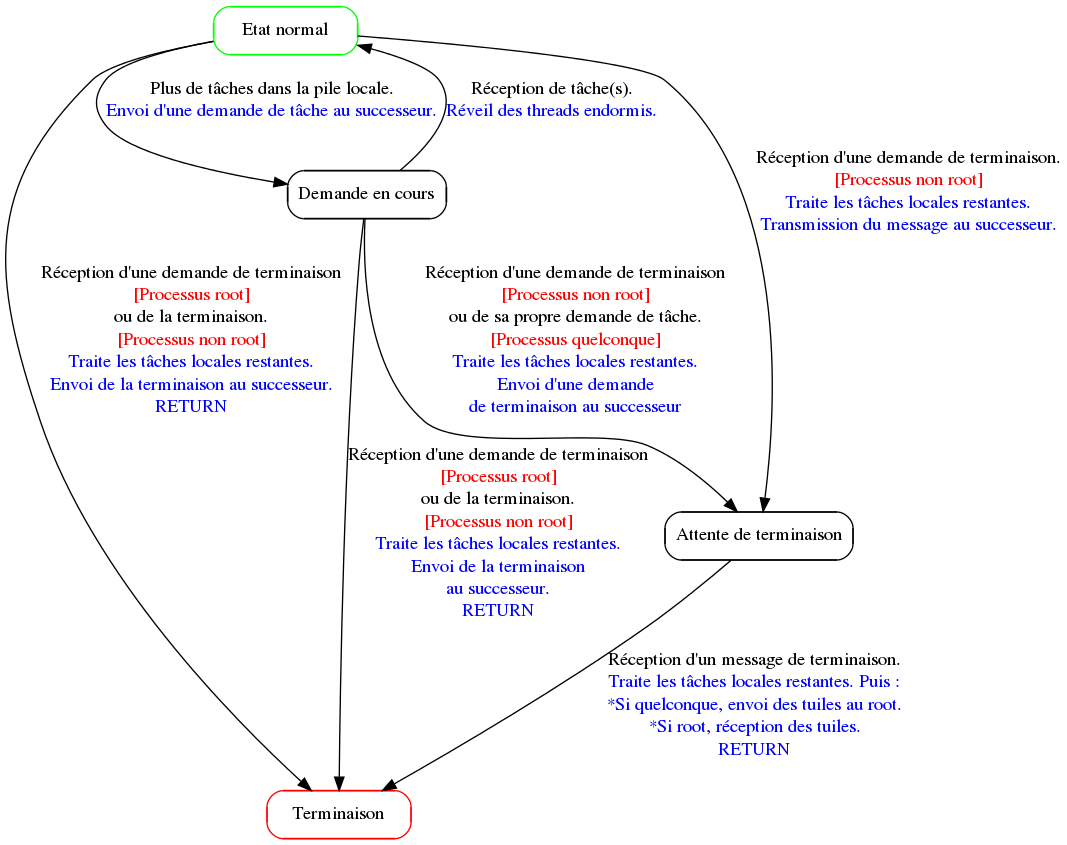
\includegraphics[scale=0.48]{automate.png}
\caption{Automate de communication, à 4 états et 4 étiquettes.}
\label{img:automate}
\end{figure}


\subsubsection*{Parallélisation avec \emph{threads}}

Afin d'augmenter la parallélisation du programme, le code exécuté par chaque processus est \emph{multithreadé}. Ainsi, les processus font tourner un \emph{thread} de communication (qui s'occupe de gérer les messages) et un certain nombre de \emph{threads} de travail (dont l'unique fonction est de traiter des tuiles).

Le code d'un \emph{thread} de travail est en fait une boucle infinie, consistant à piocher des tuiles dans la pile de tâches et à lancer les calculs dessus. Afin d'éviter les problèmes liés aux accès concurrents, nous avons protégé la pile avec un verrou. De plus, nous avons également mis en place une sémaphore afin d'endormir les \emph{threads} lorsqu'il n'y a plus de tuiles à traiter, et réciproquement afin de les réveiller lorsque de nouvelles tuiles sont disponibles.